\subsection{Test} \label{test}

Tale sezione ha lo scopo di spiegare il funzionamento, lo scopo e i risultati dei vari tipi di test proposti dal modello a V e che adottiamo.

\subsubsection{Modello a V} \label{sezionemodelloV}
Il modello a V descrive in modo sintetico il ciclo di vita della realizzazione del software, partendo dalla sua progettazione fino alla sua consegna al cliente escludendo la fase di manutenzione.

Lo scopo del modello a V è quello di mostrare quali tipi di test accompagnano ogni fase del ciclo e di come anche questi siano propedeutici l'uno dall'altro.

\begin{figure}[H]
	\centering
	%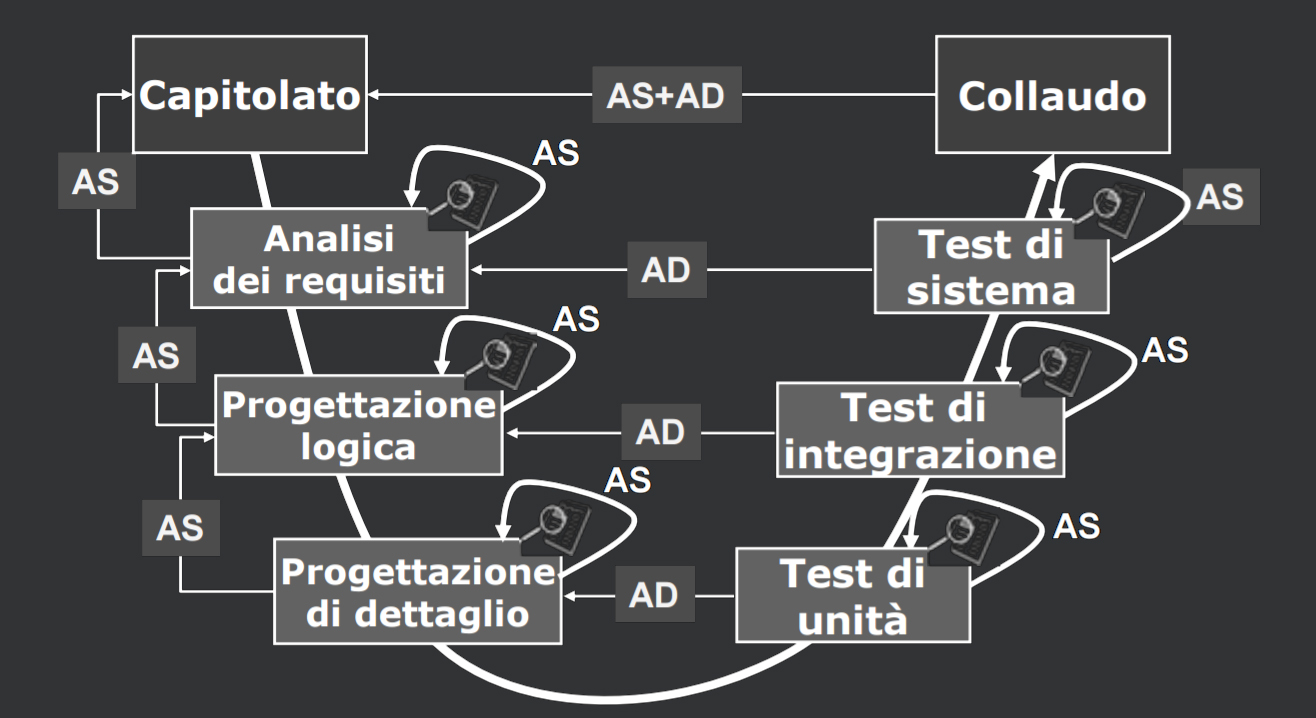
\includegraphics[width=0.8\textwidth]{img/modellov-sweki.jpg}
	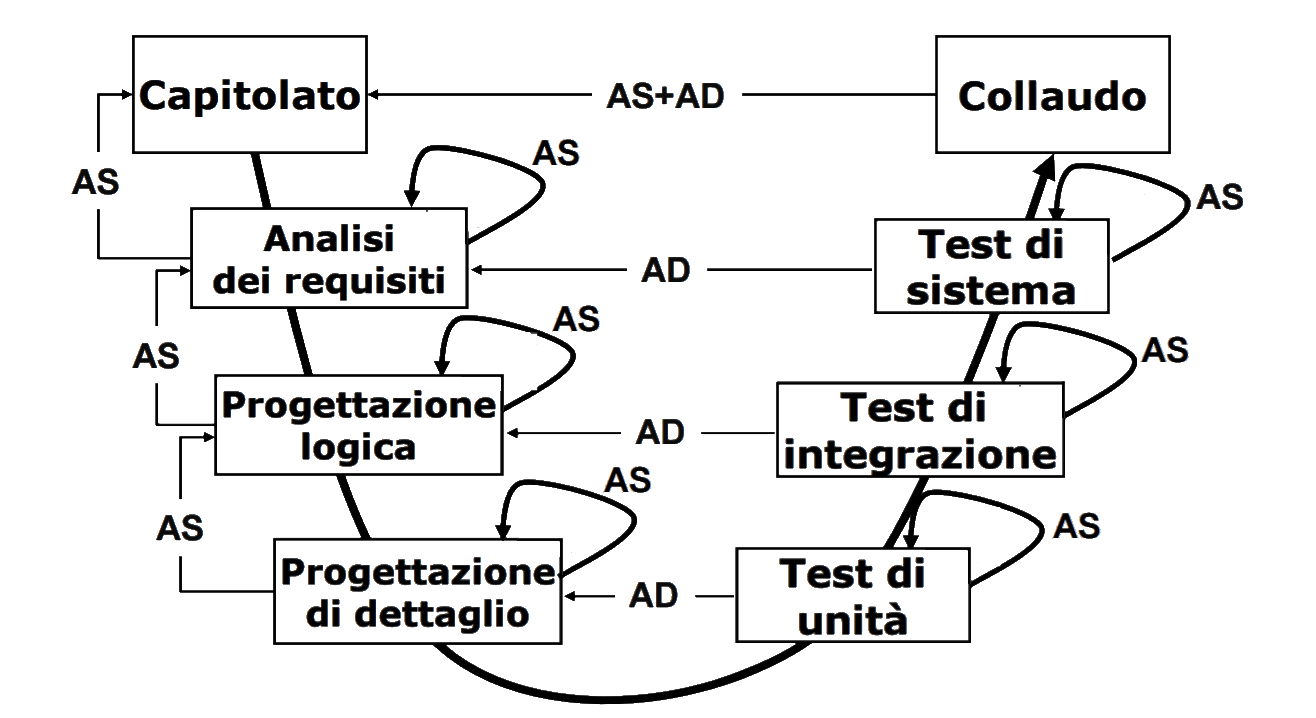
\includegraphics[width=0.8\textwidth]{img/modellov-sweki_inv.png}
	\label{img:vmodel}
	\caption[Modello a V]{Modello a V\protect\footnotemark}
\end{figure}

\footnotetext{Vedere modello a V in \S\ref{riferimenti informativi}}

\subsubsection{Classificazione e stuttura dei test} \label{classificazionetest}
Ogni test viene identificato univocamente dal seguente codice:

\begin{center}
	\texttt{T[Tipo][ID]}
\end{center}

\begin{itemize}
	\item \textbf{T}: si riferisce a ``Test''.
	\item \textbf{Tipo}: la tipologia a cui il test appartiene che, seguendo il modello a V\footnote{\url{https://en.wikipedia.org/wiki/V-Model_(software_development)}}, può essere:
	\begin{itemize}
		\item \textbf{V}: validazione. %è la stessa cosa di collaudo e di accettazione??
		\item \textbf{S}: sistema
		\item \textbf{I}: integrazione.
		\item \textbf{U}: unità.
		\end{itemize}
	%per la corrispondenza con i requisiti, non vanno bene le "tre cifre"
	\item \textbf{ID}: numero incrementale che rispetta una struttura gerarchica.
\end{itemize}

% COLORI
\newcommand{\TNI}{{\color{gray}\textbf{NI}}}
\newcommand{\TI}{{\color{blue}\textbf{I}}}
\newcommand{\TNS}{{\color{red}\textbf{NS}}}
\newcommand{\TS}{{\color{green}\textbf{S}}}

Le tabelle che raccolgono i test di una determinata tipologia presentano i campi:
\begin{itemize}
	\item \textbf{Codice}: comprendente il codice identificativo del test.
	\item \textbf{Test}: descrive cosa il test deve verificare.
	\item \textbf{Stato}: indica lo stato del test e può essere:
	\begin{itemize}
		\item \TNI: non implementato.
		\item \TI: implementato ma non ancora avviato.
		\item \TNS: avviato e fallito.
		\item \TS: avviato e superato.
	\end{itemize}
\end{itemize}

\subsubsection{Test di validazione} \label{testvalidazione}
È un tipo di test da determinare e sviluppare in parallelo con la comprensione del capitolato.
Come si può vedere dal modello a V, sono i primi tipi di test che vengono creati e saranno gli ultimi ad essere eseguiti prima della consegna del prodotto.

\newenvironment{VTtable}[1][1]{%
	\renewcommand*{\arraystretch}{#1}%
	\renewcommand\theadfont{\bfseries}%
	\oldtabularx%
}{\endoldtabularx}

\newcounter{tv}
\newcommand{\addtotv}{\stepcounter{tv}TV\thetv}

\newcounter{tableCounter}

\stepcounter{tableCounter}
\begin{table}[H]
	\begin{VTtable}[1.7]{\textwidth}{cXc}
		\rowcolor{\tablegray}
		\textbf{Codice} & \centering\textbf{Test} & \textbf{Stato} \\\toprule
		\addtotv & Verifica la segnalazione dell'apertura di una issue in Redmine:
		\begin{enumerate}
			\item Viene aperta una issue in Redmine.
			\item Redmine invia la segnalazione.
            \item Producer Redmine riceve la segnalazione da Redmine.
		\end{enumerate}
		& \TNI \\\midrule

        \addtotv & Verifica la segnalazione della modifica di una issue in Redmine:
		\begin{enumerate}
			\item Viene modificata una issue in Redmine.
			\item Redmine invia la segnalazione.
            \item Producer Redmine riceve la segnalazione da Redmine.
		\end{enumerate}
		& \TNI \\\midrule

        \addtotv & Verifica la segnalazione dell'apertura di una issue in GitLab:
		\begin{enumerate}
			\item Viene aperta una issue in GitLab.
			\item GitLab invia la segnalazione.
            \item Producer GitLab riceve la segnalazione da GitLab.
		\end{enumerate}
		& \TNI \\\midrule

        \addtotv & Verifica la segnalazione della modifica di una issue in GitLab:
		\begin{enumerate}
			\item Viene modificata una issue in GitLab.
			\item GitLab invia la segnalazione.
            \item Producer GitLab riceve la segnalazione da GitLab.
		\end{enumerate}
		& \TNI \\
        \bottomrule
	\end{VTtable}
	\caption{Elenco dei test di validazione (\thetableCounter)}
\end{table}

\stepcounter{tableCounter}
\begin{table}[H]
	\begin{VTtable}[1.7]{\textwidth}{cXc}
		\rowcolor{\tablegray}
		\textbf{Codice} & \centering\textbf{Test} & \textbf{Stato} \\\toprule
        \addtotv & Verifica di un evento di push in GitLab:
		\begin{enumerate}
			\item Viene effettuato un push su GitLab.
			\item GitLab invia la segnalazione.
            \item Producer GitLab riceve la segnalazione da GitLab.
		\end{enumerate}
		& \TNI \\\midrule

        \addtotv & Verifica di invio di un messaggio di apertura issue dal Producer Redmine al Gestore Personale:
		\begin{enumerate}
			\item Producer Redmine rielabora un messaggio di apertura issue precedentemente ricevuto.
			\item Producer Redmine invia il messaggio.
            \item Gestore personale riceve il messaggio.
		\end{enumerate}
		& \TNI \\\midrule

        \addtotv & Verifica di invio di un messaggio di modifica issue dal Producer Redmine al Gestore Personale:
		\begin{enumerate}
			\item Producer Redmine rielabora un messaggio di modifica issue precedentemente ricevuto.
			\item Producer Redmine invia il messaggio.
            \item Gestore personale riceve il messaggio.
		\end{enumerate}
		& \TNI \\\midrule

        \addtotv & Verifica di scarto di messaggi non validi nel Producer Redmine:
		\begin{enumerate}
			\item Producer Redmine riceve un messaggio di modifica issue non valido (non è stato modificato né il campo Subject né il campo Assignee).
			\item Producer Redmine scarta il messaggio.
		\end{enumerate}
		& \TNI \\\midrule

        \addtotv & Verifica di invio di un messaggio di commit dal Producer GitLab al Gestore Personale:
		\begin{enumerate}
			\item Producer GitLab rielabora une messaggio di commit.
			\item Producer GitLab invia il messaggio.
            \item Gestore personale riceve il messaggio.
		\end{enumerate}
		& \TNI \\
        \bottomrule
	\end{VTtable}
	\caption{Elenco dei test di validazione (\thetableCounter)}
\end{table}

\stepcounter{tableCounter}
\begin{table}[H]
	\begin{VTtable}[1.7]{\textwidth}{cXc}
		\rowcolor{\tablegray}
		\textbf{Codice} & \centering\textbf{Test} & \textbf{Stato} \\\toprule
        \addtotv & Verifica di invio di un messaggio di apertura issue dal Producer GitLab al Gestore Personale:
		\begin{enumerate}
			\item Producer GitLab rielabora un messaggio di apertura issue.
			\item Producer GitLab invia il messaggio.
            \item Gestore Personale riceve il messaggio.
		\end{enumerate}
		& \TNI \\\midrule

        \addtotv & Verifica di invio di un messaggio di modifica issue dal Producer GitLab al Gestore Personale:
		\begin{enumerate}
			\item Producer GitLab rielabora un messaggio di modifica issue.
			\item Producer GitLab invia il messaggio.
            \item Gestore personale riceve il messaggio.
		\end{enumerate}
		& \TNI \\\midrule

        \addtotv & Verifica di scarto di messaggi non validi nel Producer GitLab:
		\begin{enumerate}
			\item Producer GitLab riceve un messaggio di modifica issue non valido (non è stato modificato né il campo Label né il campo Title).
			\item Producer GitLab scarta il messaggio.
		\end{enumerate}
		& \TNI \\\midrule

        \addtotv & Verifica di invio di messaggi al Consumer Telegram:
		\begin{enumerate}
			\item Gestore Personale riceve un messaggio da un Producer (Redmine o GitLab).
            \item Gestore Personale rielabora il messaggio ricevuto.
			\item Gestore Personale invia il messaggio rielaborato.
            \item Consumer Telegram riceve il messaggio.
		\end{enumerate}
		& \TNI \\\midrule

        \addtotv & Verifica di invio di messaggi al Consumer Email:
		\begin{enumerate}
			\item Gestore Personale riceve un messaggio da un Producer (Redmine o GitLab).
            \item Gestore Personale rielabora il messaggio ricevuto.
			\item Gestore Personale invia il messaggio rielaborato.
            \item Consumer Email riceve il messaggio.
		\end{enumerate}
		& \TNI \\
        \bottomrule
	\end{VTtable}
	\caption{Elenco dei test di validazione (\thetableCounter)}
\end{table}

\stepcounter{tableCounter}
\begin{table}[H]
	\begin{VTtable}[1.7]{\textwidth}{cXc}
		\rowcolor{\tablegray}
		\textbf{Codice} & \centering\textbf{Test} & \textbf{Stato} \\\toprule
        \addtotv & Verifica di invio di messaggi al bot Telegram:
		\begin{enumerate}
			\item Consumer Telegram riceve un messaggio dal Gestore Personale.
			\item Consumer Telegram invia il messaggio.
            \item Bot Telegram riceve il messaggio.
		\end{enumerate}
		& \TNI \\\midrule

        \addtotv & Verifica di invio di messaggi al server Email:
		\begin{enumerate}
			\item Consumer Email riceve un messaggio dal Gestore Personale.
			\item Consumer Email invia il messaggio.
            \item Server Email riceve il messaggio.
		\end{enumerate}
		& \TNI \\\midrule

		\addtotv & Verifica di accesso di un utente al sistema tramite Email:
		\begin{enumerate}
			\item Inserire nel Gestore Personale l'Email dell'utente
			\item Confermare l'invio dei dati.
            \item L'accesso al sistema è avvenuto correttamente.
		\end{enumerate}
		& \TNI \\\midrule

        \addtotv & Verifica di accesso di un utente al sistema tramite ID Telegram:
		\begin{enumerate}
			\item Inserire nel Gestore Personale l'ID Telegram dell'utente
			\item Confermare l'invio dei dati.
            \item L'accesso al sistema è avvenuto correttamente.
		\end{enumerate}
		& \TNI \\\midrule

        \addtotv & Verifica di errore per accesso con Email inesistente:
		\begin{enumerate}
			\item Inserire nel Gestore Personale l'Email dell'utente
			\item Confermare l'invio dei dati.
            \item Viene segnalato un errore.
		\end{enumerate}
		& \TNI \\
        \bottomrule
	\end{VTtable}
	\caption{Elenco dei test di validazione (\thetableCounter)}
\end{table}

\stepcounter{tableCounter}
\begin{table}[H]
	\begin{VTtable}[1.7]{\textwidth}{cXc}
		\rowcolor{\tablegray}
		\textbf{Codice} & \centering\textbf{Test} & \textbf{Stato} \\\toprule
        \addtotv & Verifica di errore per accesso con ID Telegram inesistente:
		\begin{enumerate}
			\item Inserire nel Gestore Personale l'ID Telegram dell'utente
			\item Confermare l'invio dei dati.
            \item Viene segnalato un errore.
		\end{enumerate}
		& \TNI \\\midrule

        \addtotv & Verifica di uscita dell'utente dal sistema:
		\begin{enumerate}
			\item Confermare l'uscita dal sistema.
            \item L'utente viene riportato all'accesso al sistema.
		\end{enumerate}
		& \TNI \\ \midrule

        \addtotv & Verifica di registrazione di un nuovo utente:
		\begin{enumerate}
			\item Accedere al sistema (utente non registrato).
            \item Inserire i seguenti campi:
                \begin{itemize}
                    \item Nome
                    \item Cognome
                    \item Contatto Email
                    \item Contatto Telegram
                \end{itemize}
            \item Confermare l'invio dei dati.
            \item L'utente viene registrato correttamente.
		\end{enumerate}
		& \TNI \\\midrule

        \addtotv & Verifica di errore per Email già esistente:
		\begin{enumerate}
			\item Accedere al sistema.
            \item Inserire i seguenti campi:
                \begin{itemize}
                    \item Nome
                    \item Cognome
                    \item Contatto Email
                    \item Contatto Telegram
                \end{itemize}
            \item Confermare l'invio dei dati.
            \item Viene segnalato un errore.
		\end{enumerate}
		& \TNI \\
        \bottomrule
	\end{VTtable}
	\caption{Elenco dei test di validazione (\thetableCounter)}
\end{table}

\stepcounter{tableCounter}
\begin{table}[H]
	\begin{VTtable}[1.7]{\textwidth}{cXc}
		\rowcolor{\tablegray}
		\textbf{Codice} & \centering\textbf{Test} & \textbf{Stato} \\\toprule
        \addtotv & Verifica di errore per ID Telegram già esistente:
		\begin{enumerate}
			\item Accedere al sistema (utente non registrato).
            \item Inserire i seguenti campi:
                \begin{itemize}
                    \item Nome
                    \item Cognome
                    \item Contatto Email
                    \item Contatto Telegram
                \end{itemize}
            \item Confermare l'invio dei dati.
            \item Viene segnalato un errore.
		\end{enumerate}
		& \TNI \\\midrule

        \addtotv & Verifica di rimozione di un utente dal sistema tramite Telegram:
		\begin{enumerate}
			\item Accedere al sistema.
            \item Inserire l'ID Telegram dell'utente da rimuovere.
            \item Confermare l'invio dei dati.
            \item L'utente è stato correttamente rimosso dal sistema.
		\end{enumerate}
		& \TNI \\ \\\midrule

        \addtotv & Verifica di rimozione di un utente dal sistema tramite Email:
		\begin{enumerate}
			\item Accedere al sistema.
            \item Inserire l'Email dell'utente da rimuovere.
            \item Confermare l'invio dei dati.
            \item L'utente è stato correttamente rimosso dal sistema.
		\end{enumerate}
		& \TNI \\\midrule

        \addtotv & Verifica di errore nella rimozione di un utente con Email inesistente dal sistema:
		\begin{enumerate}
			\item Accedere al sistema.
            \item Inserire l'Email dell'utente da rimuovere.
            \item Confermare l'invio dei dati.
            \item Viene segnalato un errore.
		\end{enumerate}
		& \TNI \\
        \bottomrule
	\end{VTtable}
	\caption{Elenco dei test di validazione (\thetableCounter)}
\end{table}

\stepcounter{tableCounter}
\begin{table}[H]
	\begin{VTtable}[1.7]{\textwidth}{cXc}
		\rowcolor{\tablegray}
		\textbf{Codice} & \centering\textbf{Test} & \textbf{Stato} \\\toprule

        \addtotv & Verifica di errore nella rimozione di un utente con ID Telegram inesistente dal sistema:
		\begin{enumerate}
			\item Accedere al sistema.
            \item Inserire l'ID Telegram dell'utente da rimuovere.
            \item Confermare l'invio dei dati.
            \item Viene segnalato un errore.
		\end{enumerate}
		& \TNI \\\midrule

        \addtotv & Verifica di rimozione dell'utente acceduto dal sistema tramite Email:
		\begin{enumerate}
			\item Accedere al sistema.
            \item Inserire la propria Email.
            \item Confermare l'invio dei dati.
            \item Si esce dal sistema e si viene riportati alla schermata di accesso.
		\end{enumerate}
		& \TNI \\\midrule

        \addtotv & Verifica di rimozione dell'utente acceduto dal sistema tramite ID Telegram:
		\begin{enumerate}
			\item Accedere al sistema.
            \item Inserire la propria Email.
            \item Confermare l'invio dei dati.
            \item Si esce dal sistema e si viene riportati alla schermata di accesso.
		\end{enumerate}
		& \TNI \\
        \bottomrule
	\end{VTtable}
	\caption{Elenco dei test di validazione (\thetableCounter)}
\end{table}

\stepcounter{tableCounter}
\begin{table}[H]
	\begin{VTtable}[1.7]{\textwidth}{cXc}
		\rowcolor{\tablegray}
		\textbf{Codice} & \centering\textbf{Test} & \textbf{Stato} \\\toprule
        \addtotv & Verifica di modifica di un utente tramite Email:
		\begin{enumerate}
			\item Accedere al sistema.
            \item Inserire i seguenti campi:
                \begin{itemize}
                    \item Email dell'utente da modificare
                    \item Nome
                    \item Cognome
                    \item Contatto Email
                    \item Contatto Telegram
                \end{itemize}
            \item Confermare l'invio dei dati.
            \item L'utente è stato modificato correttamente.
		\end{enumerate}
		& \TNI \\\midrule

        \addtotv & Verifica di modifica di un utente tramite ID Telegram:
		\begin{enumerate}
			\item Accedere al sistema.
            \item Inserire i seguenti campi:
                \begin{itemize}
                    \item Email dell'utente da modificare
                    \item Nome
                    \item Cognome
                    \item Contatto Email
                    \item Contatto Telegram
                \end{itemize}
            \item Confermare l'invio dei dati.
            \item L'utente è stato modificato correttamente.
		\end{enumerate}
		& \TNI \\
        \bottomrule
	\end{VTtable}
	\caption{Elenco dei test di validazione (\thetableCounter)}
\end{table}

\stepcounter{tableCounter}
\begin{table}[H]
	\begin{VTtable}[1.7]{\textwidth}{cXc}
		\rowcolor{\tablegray}
		\textbf{Codice} & \centering\textbf{Test} & \textbf{Stato} \\\toprule
        \addtotv & Verifica di errore nella modifica di un utente con Email già esistente tramite Email:
		\begin{enumerate}
			\item Accedere al sistema.
            \item Inserire i seguenti campi:
                \begin{itemize}
                    \item Email dell'utente da modificare
                    \item Nome
                    \item Cognome
                    \item Contatto Email già esistente
                    \item Contatto Telegram
                \end{itemize}
            \item Confermare l'invio dei dati.
            \item Viene segnalato un errore.
		\end{enumerate}
		& \TNI \\\midrule

        \addtotv & Verifica di errore nella modifica di un utente con ID Telegram già esistente tramite Email:
		\begin{enumerate}
			\item Accedere al sistema.
            \item Inserire i seguenti campi:
                \begin{itemize}
                    \item Email dell'utente da modificare
                    \item Nome
                    \item Cognome
                    \item Contatto Email
                    \item Contatto Telegram già esistente
                \end{itemize}
            \item Confermare l'invio dei dati.
            \item Viene segnalato un errore.
		\end{enumerate}
		& \TNI \\
        \bottomrule
	\end{VTtable}
	\caption{Elenco dei test di validazione (\thetableCounter)}
\end{table}

\stepcounter{tableCounter}
\begin{table}[H]
	\begin{VTtable}[1.7]{\textwidth}{cXc}
		\rowcolor{\tablegray}
		\textbf{Codice} & \centering\textbf{Test} & \textbf{Stato} \\\toprule
        \addtotv & Verifica di errore nella modifica di un utente con Email già esistente tramite ID Telegram:
		\begin{enumerate}
			\item Accedere al sistema.
            \item Inserire i seguenti campi:
                \begin{itemize}
                    \item ID Telegram dell'utente da modificare
                    \item Nome
                    \item Cognome
                    \item Contatto Email già esistente
                    \item Contatto Telegram
                \end{itemize}
            \item Confermare l'invio dei dati.
            \item Viene segnalato un errore.
		\end{enumerate}
		& \TNI \\\midrule

        \addtotv & Verifica di errore nella modifica di un utente con ID Telegram già esistente tramite ID Telegram:
		\begin{enumerate}
			\item Accedere al sistema.
            \item Inserire i seguenti campi:
                \begin{itemize}
                    \item ID Telegram dell'utente da modificare
                    \item Nome
                    \item Cognome
                    \item Contatto Email
                    \item Contatto Telegram già esistente
                \end{itemize}
            \item Confermare l'invio dei dati.
            \item Viene segnalato un errore.
		\end{enumerate}
		& \TNI \\
        \bottomrule
	\end{VTtable}
	\caption{Elenco dei test di validazione (\thetableCounter)}
\end{table}

\stepcounter{tableCounter}
\begin{table}[H]
	\begin{VTtable}[1.7]{\textwidth}{cXc}
		\rowcolor{\tablegray}
		\textbf{Codice} & \centering\textbf{Test} & \textbf{Stato} \\\toprule
        \addtotv & Verifica di errore nella modifica di un utente con Email inesistente:
		\begin{enumerate}
			\item Accedere al sistema.
            \item Inserire i seguenti campi:
                \begin{itemize}
                    \item Email dell'utente da modificare non esistente
                    \item Nome
                    \item Cognome
                    \item Contatto Email
                    \item Contatto Telegram
                \end{itemize}
            \item Confermare l'invio dei dati.
            \item Viene segnalato un errore.
		\end{enumerate}
		& \TNI \\\midrule

        \addtotv & Verifica di errore nella modifica di un utente con ID Telegram inesistente:
		\begin{enumerate}
			\item Accedere al sistema.
            \item Inserire i seguenti campi:
                \begin{itemize}
                    \item ID Telegram dell'utente da modificare non esistente
                    \item Nome
                    \item Cognome
                    \item Contatto Email
                    \item Contatto Telegram
                \end{itemize}
            \item Confermare l'invio dei dati.
            \item Viene segnalato un errore.
		\end{enumerate}
		& \TNI \\\midrule

        \addtotv & Verifica di iscrizione a un nuovo topic:
		\begin{enumerate}
			\item Accedere al sistema.
            \item Selezionare un nuovo topic a cui iscriversi.
            \item Confermare l'invio dei dati.
            \item Il topic è stato correttamente aggiunto alle preferenze dell'utente.
		\end{enumerate}
		& \TNI \\
        \bottomrule
	\end{VTtable}
	\caption{Elenco dei test di validazione (\thetableCounter)}
\end{table}

\stepcounter{tableCounter}
\begin{table}[H]
	\begin{VTtable}[1.7]{\textwidth}{cXc}
		\rowcolor{\tablegray}
		\textbf{Codice} & \centering\textbf{Test} & \textbf{Stato} \\\toprule
        \addtotv & Verifica di aggiunta dei giorni di indisponibilità al calendario:
		\begin{enumerate}
			\item Accedere al sistema.
            \item Selezionare i giorni di indisponibilità da aggiungere.
            \item Confermare l'invio dei dati.
            \item I giorni sono stati aggiunti correttamente alle preferenze dell'utente.
		\end{enumerate}
		& \TNI \\\midrule

        \addtotv & Verifica di aggiunta della piattaforma di messaggistica preferita:
		\begin{enumerate}
			\item Accedere al sistema.
            \item Selezionare la piattaforma preferita per la ricezione dei messaggi da aggiungere.
            \item Confermare l'invio dei dati.
            \item La piattaforma è stata correttamente aggiunta alle preferenze dell'utente.
		\end{enumerate}
		& \TNI \\\bottomrule
	\end{VTtable}
	\caption{Elenco dei test di validazione (\thetableCounter)}
\end{table}

\stepcounter{tableCounter}
\begin{table}[H]
	\begin{VTtable}[1.7]{\textwidth}{cXc}
		\rowcolor{\tablegray}
		\textbf{Codice} & \centering\textbf{Test} & \textbf{Stato} \\\toprule
        \addtotv & Verifica di aggiunta delle keyword per i push di GitLab:
		\begin{enumerate}
			\item Accedere al sistema.
            \item Aggiungere le keyword GitLab.
            \item Confermare l'invio dei dati.
            \item Le keyword di GitLab sono state aggiornate correttamente.
		\end{enumerate}
		& \TNI \\\midrule

        \addtotv & Verifica di errore nell'aggiunta delle keyword per i push di GitLab già esistenti:
		\begin{enumerate}
			\item Accedere al sistema.
            \item Aggiungere delle keyword GitLab già presenti.
            \item Confermare l'invio dei dati.
            \item Viene segnalato un errore.
		\end{enumerate}
		& \TNI \\\midrule

        \addtotv & Verifica di rimozione di un topic:
		\begin{enumerate}
			\item Accedere al sistema.
            \item Selezionare un topic da rimuovere.
            \item Confermare l'invio dei dati.
            \item Il topic è stato rimosso correttamente dalle preferenze.
		\end{enumerate}
		& \TNI \\\midrule

        \addtotv & Verifica di rimozione dei giorni di indisponibilità dal calendario:
		\begin{enumerate}
			\item Accedere al sistema.
            \item Selezionare i giorni di indisponibilità da rimuovere.
            \item Confermare l'invio dei dati.
            \item I giorni sono stati rimossi dalle preferenze correttamente.
		\end{enumerate}
		& \TNI \\
        \bottomrule
	\end{VTtable}
	\caption{Elenco dei test di validazione (\thetableCounter)}
\end{table}

\stepcounter{tableCounter}
\begin{table}[H]
	\begin{VTtable}[1.7]{\textwidth}{cXc}
		\rowcolor{\tablegray}
		\textbf{Codice} & \centering\textbf{Test} & \textbf{Stato} \\\toprule

        \addtotv & Verifica di rimozione della piattaforma di messaggistica preferita:
		\begin{enumerate}
			\item Accedere al sistema.
            \item Selezionare la piattaforma preferita per la ricezione dei messaggi da rimuovere.
            \item Confermare l'invio dei dati.
            \item La piattaforma è stata correttamente rimossa dalle preferenze.
		\end{enumerate}
		& \TNI \\\midrule

        \addtotv & Verifica di rimozione delle keyword per i push di GitLab:
		\begin{enumerate}
			\item Accedere al sistema.
            \item Aggiungere le keyword GitLab.
            \item Confermare l'invio dei dati.
            \item Le keyword GitLab sono state aggiornate correttamente.
		\end{enumerate}
		& \TNI \\
        \bottomrule
	\end{VTtable}
	\caption{Elenco dei test di validazione (\thetableCounter)}
\end{table}

\stepcounter{tableCounter}
\begin{table}[H]
	\begin{VTtable}[1.7]{\textwidth}{cXc}
		\rowcolor{\tablegray}
		\textbf{Codice} & \centering\textbf{Test} & \textbf{Stato} \\\toprule

        \addtotv & Verifica di errore nella rimozione delle keyword inesistenti per i push di GitLab:
		\begin{enumerate}
			\item Accedere al sistema.
            \item Aggiungere delle keyword GitLab non presenti.
            \item Confermare l'invio dei dati.
            \item Viene segnalato un errore.
		\end{enumerate}
		& \TNI \\
        \bottomrule
	\end{VTtable}
	\caption{Elenco dei test di validazione (\thetableCounter)}
\end{table}

\newpage

	\paragraph{Tracciamento} \label{tracciamentovalidazione}

    \setcounter{tv}{0}

	\setcounter{tableCounter}{1}
	\begin{table}[H]
		\centering
		{\def\arraystretch{1.4}
		\begin{tabularx}{\textwidth}{YY}
			% \rowcolor{\tablegray}
			\textbf{Codice} & \textbf{Requisito} \\
			\toprule
			\addtotv &  \\
			\addtotv &  \\
			\addtotv &  \\
			\addtotv &  \\
			\addtotv &  \\
			\addtotv &  \\
			\addtotv &  \\
			\addtotv &  \\
			\addtotv & \\
			\addtotv &  \\
			\addtotv &  \\
			\addtotv & \\
			\addtotv & \\
			\addtotv & \\
			\addtotv & \\
			\addtotv & \\
			\addtotv &  \\
			\addtotv &  \\
			\addtotv & \\
			\addtotv & \\
			\addtotv & \\
			\addtotv & \\
			\addtotv &  \\
			\addtotv &  \\
			\addtotv &  \\
			\addtotv &  \\
			\addtotv &  \\
			\addtotv &  \\
			\addtotv &  \\
			\addtotv &  \\
			\addtotv &  \\
            \bottomrule
            \end{tabularx}}
		\caption{Elenco dei test in correlazioni con i requisiti (\thetableCounter)}
	\end{table}

	\stepcounter{tableCounter}
    \begin{table}[H]
		\centering
		{\def\arraystretch{1.4}
		\begin{tabularx}{\textwidth}{YY}
			% \rowcolor{\tablegray}
			\textbf{Codice} & \textbf{Requisito} \\
			\toprule
            \addtotv & \\
			\addtotv & \\
			\addtotv &  \\
			\addtotv &  \\
			\addtotv &  \\
			\addtotv &  \\
			\addtotv & \\
			\addtotv & \\
			\addtotv & \\
			\addtotv & \\
			\addtotv & \\
			\addtotv &  \\
			\addtotv & \\
			\addtotv &  \\
			\addtotv & \\
			\addtotv & \\
			\addtotv & \\
			\bottomrule
		\end{tabularx}}
		\caption{Elenco dei test in correlazioni con i requisiti (\thetableCounter)}
	\end{table}

\newpage

\newcounter{ts}
\newcommand{\addtots}{\stepcounter{ts}TS\thets}

\subsubsection{Test di sistema} \label{testsistema}
Tipo di test da scegliere durante l'attività di analisi dei requisiti. Servono per svolgere la validazione del prodotto.

I test di sistema servono per testare l'intero prodotto, in particolare le sue specifiche tecniche e funzionali.
Per questo si creano dei test derivanti dai casi d'uso e dai requisiti funzionali presenti nell'\AdRd.

\setcounter{tableCounter}{1}
\begin{table}[H]
	\begin{paddedtablex}[1.7]{\textwidth}{cXc}
		% \rowcolor{\tablegray}
		\textbf{Codice} & \centering\textbf{Test} & \textbf{Stato} \\\toprule
        \addtots & Verifica che il sistema riceva la segnalazione dell'apertura di una issue da parte di Redmine & \TNI \\
        \addtots & Verifica che il sistema riceva la segnalazione della modifica di una issue da parte di Redmine & \TNI \\
        \addtots & Verifica che il sistema riceva la segnalazione dell'apertura di una issue da parte di GitLab & \TNI \\
        \addtots & Verifica che il sistema riceva la segnalazione della modifica di una issue da parte di GitLab & \TNI \\
        \addtots & Verifica che il sistema riceva eventi di push da parte di GitLab & \TNI \\
		\addtots & Verifica di invio di un messaggio di apertura issue dal Producer Redmine al Gestore Personale & \TNI \\
		\addtots & Verifica di invio di un messaggio di modifica issue dal Producer Redmine al Gestore Personale & \TNI \\
		\addtots & Verifica di scarto di messaggi non validi nel Producer Redmine & \TNI \\
		\addtots & Verifica di invio di un messaggio di commit dal Producer GitLab al Gestore Personale & \TNI \\
        \addtots & Verifica di invio di un messaggio di apertura issue dal Producer GitLab al Gestore Personale & \TNI \\
        \addtots & Verifica di invio di un messaggio di modifica issue dal Producer GitLab al Gestore Personale & \TNI \\
        \addtots & Verifica di scarto di messaggi non validi nel Producer GitLab & \TNI \\
        \addtots & Verifica di invio di messaggi al Consumer Telegram & \TNI \\
        \addtots & Verifica di invio di messaggi al Consumer Email & \TNI \\
        \addtots & Verifica di invio di messaggi al bot Telegram & \TNI \\
        \bottomrule
	\end{paddedtablex}
	\caption{Elenco dei test di sistema (\thetableCounter)}
\end{table}

\stepcounter{tableCounter}
\begin{table}[H]
	\begin{paddedtablex}[1.7]{\textwidth}{cXc}
		% \rowcolor{\tablegray}
		\textbf{Codice} & \centering\textbf{Test} & \textbf{Stato} \\\toprule
        \addtots & Verifica di invio di messaggi al server Email & \TNI \\
        \addtots & Verifica di accesso di un utente al sistema tramite Email & \TNI \\
        \addtots & Verifica di accesso di un utente al sistema tramite ID Telegram & \TNI \\
        \addtots & Verifica di errore per accesso con Email inesistente & \TNI \\
        \addtots & Verifica di errore per accesso con ID Telegram inesistente & \TNI \\
        \addtots & Verifica di uscita dell'utente dal sistema & \TNI \\
        \addtots & Verifica di registrazione di un nuovo utente & \TNI \\
        \addtots & Verifica di errore per Email già esistente & \TNI \\
        \addtots & Verifica di errore per ID Telegram già esistente & \TNI \\
        \addtots & Verifica di rimozione utente dal sistema tramite Telegram & \TNI \\
        \addtots & Verifica di rimozione utente dal sistema tramite Email & \TNI \\
        \addtots & Verifica di errore nella rimozione di un utente con Email inesistente dal sistema & \TNI \\
        \addtots & Verifica di errore nella rimozione di un utente con ID Telegram inesistente dal sistema & \TNI \\
        \addtots & Verifica di rimozione dell'utente acceduto dal sistema tramite Email & \TNI \\
        \addtots & Verifica di rimozione dell'utente acceduto dal sistema tramite ID Telegram & \TNI \\
        \addtots & Verifica di modifica di un utente tramite Email & \TNI \\
        \addtots & Verifica di modifica di un utente tramite ID Telegram & \TNI \\
        \addtots & Verifica di errore nella modifica di un utente con Email già esistente tramite Email & \TNI \\
        \addtots & Verifica di errore nella modifica di un utente con ID Telegram già esistente tramite Email & \TNI \\
        \addtots & Verifica di errore nella modifica di un utente con Email già esistente tramite ID Telegram & \TNI \\
        \addtots & Verifica di errore nella modifica di un utente con ID Telegram già esistente tramite ID Telegram & \TNI \\
        \addtots & Verifica di errore nella modifica di un utente con Email inesistente & \TNI \\
        \addtots & Verifica di errore nella modifica di un utente con ID Telegram inesistente & \TNI \\
        \bottomrule
	\end{paddedtablex}
	\caption{Elenco dei test di sistema (\thetableCounter)}
\end{table}

\stepcounter{tableCounter}
\begin{table}[H]
	\begin{paddedtablex}[1.7]{\textwidth}{cXc}
		\rowcolor{white}\textbf{Codice} & \centering\textbf{Test} & \textbf{Stato} \\\toprule
        \rowcolor{\tablegray}\addtots & Verifica di iscrizione a un nuovo topic & \TNI \\
        \rowcolor{white}\addtots & Verifica di aggiunta dei giorni di indisponibilità al calendario & \TNI \\
		\rowcolor{\tablegray}\addtots & Verifica di aggiunta della piattaforma di messaggistica preferita & \TNI \\
        \rowcolor{white}\addtots & Verifica di aggiunta delle keyword per i push di GitLab & \TNI \\
        \rowcolor{\tablegray}\addtots & Verifica di errore nell'aggiunta delle keyword per i push di GitLab già esistenti & \TNI \\
        \rowcolor{white}\addtots & Verifica di rimozione di un topic & \TNI \\
        \rowcolor{\tablegray}\addtots & Verifica di rimozione dei giorni di indisponibilità dal calendario & \TNI \\
        \rowcolor{white}\addtots & Verifica di rimozione della piattaforma di messaggistica preferita & \TNI \\
        \rowcolor{\tablegray}\addtots & Verifica di rimozione delle keyword per i push di GitLab & \TNI \\
        \rowcolor{white}\addtots & Verifica di errore nella rimozione delle keyword inesistenti per i push di GitLab & \TNI \\

		\bottomrule
	\end{paddedtablex}
	\caption{Elenco dei test di sistema (\thetableCounter)}
\end{table}


%Per ogni test vengono affrontati i seguenti punti:
%
%\begin{itemize}
%	\item \textbf{Scopo}: lo scopo del test che; il titolo del punto non verrà inserito nei paragrafi dei test. 
%	\item \textbf{Procedura}: vengono descritti i passaggi da compiere per eseguire il test.
%	\item \textbf{Approvazione}: vengono descritte le condizioni affinché il test sia considerato superato.
%\end{itemize}
%
%Alcuni termini ed espressioni assumono il seguente significato:
%
%\begin{itemize}
%	\item \textbf{Piattaforma di messaggistica}: s'intende sempre Telegram ed Email.
%	\item \textbf{Notifica}: s'intende una notifica in una delle piattaforme di messaggistica causata dall'applicazione.
%	\item \textbf{Topic}: s'intende l'insieme delle etichette delle issue di GitLab e Redmine e delle keyword presenti nei messaggi di commit notificati dai push di GitLab.
%	\item \textbf{Persona delegata}: s'intende l'utente a cui verranno inoltrate le notifiche nei giorni di indisponibilità dell'utente che sta usando l'applicazione.
%\end{itemize}

		%\paragraph*{Accettazione}
		%Il nuovo utente deve comparire all'interno della lista degli utenti inseriti nell'applicazione.

%	\subsubsection{TS002 Iscrizione ad una label, ad una piattaforma di messaggistica e apertura issue}
%		Un utente quando s'iscrive ad una label, lo fa con l'intenzione di ricevere le notifiche inerenti solo a quella label provenienti da GitLab o Redmine e l'iscrizione alla piattaforma di messaggistica (Telegram o Email) per scegliere dove ricevere tali notifiche.
%
%		\paragraph*{Procedura}
%			\begin{enumerate}
%				\item Selezionare l'utente con cui si vuole usare l'applicativo.
%				\item Selezionare la label da cui si vuole ricevere le notifiche. Dalle label è possibile capire quali notifiche derivano da Redmine e quali da GitLab.
%				\item Selezionare Telegram o Email per decidere in che piattaforma di messaggistica ricevere le notifiche della label.
%				\item Aprire una issue da GitLab se l'iscrizione è stata fatta da una label proveniente da GitLab, o aprire una issue da Redmine se l'iscrizione è stata fatta da una label proveniente da Redmine.
%			\end{enumerate}
%
%		\paragraph*{Accettazione}
%		Alla piattaforma di messaggistica selezionata arriva una notifica dell'apertura della issue inerente al topic selezionato.
%
%	\subsubsection{TS003 Iscrizione a una label, a una piattaforma di messaggistica e modifica issue}
%		Come descritto nel test precedente, un utente può iscriversi a una label e a una piattaforma di messaggistica per ricevere una notifica.
%
%		\paragraph*{Procedura}
%			\begin{enumerate}
%				\item Selezionare l'utente con cui si vuole usare l'applicativo.
%				\item Selezionare la label da cui si vuole ricevere le notifiche. Dalla label è possibile capire quali derivano da Redmine e quali da GitLab.
%				\item Selezionare Telegram o Email per decidere in che piattaforma di messaggistica ricevere le notifiche delle label.
%				\item Selezionare su Redmine, se ci si è iscritti ad una label di Redmine, o su GitLab, se ci si è inscritti ad una label su GitLab, una issue già aperta e modificarla in termini di label o titolo della issue.
%				\item Se tra i campi modificati nella issue ci sono anche le label, iscriversi nel Gestore Personale alla label della issue modificata.
%			\end{enumerate}
%
%		\paragraph*{Accettazione}
%		La modifica del titolo o delle label di una issue di Redmine o GitLab comporta l'invio della notifica a tutti gli iscritti alle nuove label, se queste sono cambiate, altrimenti agli iscritti delle solite label se è cambiato solo il titolo della issue. La modifica di qualsiasi altro campo non comporta l'invio di una notifica.
%
%	\subsubsection{TS004 Disiscrizione da una label}
%		La disiscrizione ad una label deve terminare la notifica delle segnalazioni legate a quella label.
%
%		\paragraph*{Procedura}
%			\begin{enumerate}
%				\item Selezionare l'utente con cui si vuole usare l'applicativo.
%				\item Disiscriversi da una label a cui precedentemente si era iscritti.
%				\item Aprire o modificare una issue da Redmine o GitLab con la label da cui ci si è disiscritti precedentemente.
%			\end{enumerate}
%
%		\paragraph*{Accettazione}
%		Una volta disiscritti ad una label non vengono più ricevute notifica riguardanti quella label.
%
%	\subsubsection{TS005 Aggiunta di una keyword, iscrizione ad una piattaforma di messaggistica e push di GitLab}
%		Per ricevere le notifiche dei push di GitLab è possibile selezionare delle keyword che possono essere presenti nei messaggi di commit.
%
%		\paragraph*{Procedura}
%		\begin{itemize}
%			\item Selezionare l'utente con cui si vuole usare l'applicativo.
%			\item Aggiungere una keyword nel Gestore Personale.
%			\item Effettuare un push su GitLab dove il messaggio di commit contiene la keyword appena inserita.
%		\end{itemize}
%
%		\paragraph*{Accettazione}
%		L'utente le notifiche dei push che nel loro messaggio di commit contengo la keyword aggiunta.
%
%	\subsubsection{TS006 Rimozione di una keyword}
%		La rimozione di una delle keyword aggiunta precedentemente evita di ricevere la notifica dei push di GitLab con il messaggio di commit con la keyword rimossa.
%
%		\paragraph*{Procedura}
%			\begin{enumerate}
%				\item Selezionare l'utente con cui si vuole usare l'applicativo.
%				\item Rimuovere una delle keyword selezionate in precedenza.
%				\item Effettuare un push su GitLab dove il messaggio di commit contiene la keyword appena rimossa.
%			\end{enumerate}
%
%		\paragraph*{Accettazione}
%		Non arrivano le notifiche dei push di GitLab in cui nel messaggio di commit è presente la keyword appena rimossa.
%
%	\subsubsection{TS007 Rimozione di una piattaforma di messaggistica}
%		Come per il test precedente, anche rimuovendo una piattaforma di messaggistica (Telegram o Email), le notifiche a quella piattaforma non dovrebbero più arrivare.
%
%		\paragraph*{Procedura}
%		\begin{enumerate}
%			\item Selezionare l'utente con cui si vuole usare l'applicativo.
%			\item Deselezionare una piattaforma di messaggistica precedentemente selezionata
%			\item Creare o modificare una issue da Redmine o GitLab, oppure effettuare un \gloss{push}.
%		\end{enumerate}
%
%		\paragraph*{Accettazione}
%		Dopo aver aperto una issue o effettuato un push da GitLab o Redmine, non si ricevono più notifiche dalle piattaforme di messaggistica rimosse.
%
%	\subsubsection{TS008 Aggiunta della persona delegata e dei giorni di indisponibilità}
%		All'interno del Gestore Personale è possibile indicare i giorni di calendario in cui si è irreperibili ed è possibile selezionare una persona a cui inoltrare le notifiche che arrivano nei giorni selezionati.
%
%		\paragraph*{Procedura}
%			\begin{enumerate}
%				\item Selezionare l'utente con cui si vuole usare l'applicativo.
%				\item Aggiungere nel Gestore Personale il giorno di esecuzione del test come giorno di indisponibilità in cui non si vogliono ricevere notifiche dall'applicativo.
%				\item Aggiungere, tra gli utenti inseriti nell'applicazione, l'utente a cui inoltrare le notifiche nei giorni di indisponibilità.
%				\item Creare o modificare una issue da Redmine o GitLab, oppure effettuare un \gloss{push}.
%			\end{enumerate}
%
%		\paragraph*{Accettazione}
%		La persona delegata riceve la notifica del messaggio che sarebbe dovuta arrivare all'utente che non è disponibile.
%
%	\subsubsection{TS009 Rimozione giorni di indisponibilità}
%		Nel momento in cui si rimuovono i giorni in cui ci si considera non reperibili, le notifiche dei topic a cui ci si è iscritti tornano ad essere inviate.
%
%		\paragraph*{Procedura}
%			\begin{enumerate}
%				\item Selezionare l'utente con cui si vuole usare l'applicativo.
%				\item Deselezionare tra i giorni di irreperibilità il giorno di esecuzione del test (se il giorno è già selezionato, selezionarlo e poi deselezionarlo).
%				\item Effettuare un push da GitLab oppure aprire o modificare una issue su Redmine o GitLab.
%			\end{enumerate}
%
%		\paragraph*{Accettazione}
%		L'utente selezionato ricomincia a ricevere notifiche.

	\paragraph{Tracciamento}

    \setcounter{ts}{0}

	\setcounter{tableCounter}{1}
	\begin{table}[H]
		\centering
		{\def\arraystretch{1.4}
		\begin{tabularx}{\textwidth}{YY}
			% \rowcolor{\tablegray}
			\textbf{Codice} & \textbf{Requisito} \\
			\toprule
			\addtots & \\
			\addtots & \\
			\addtots & \\
			\addtots & \\
			\addtots & \\
			\addtots & \\
			\addtots &  \\
			\addtots & \\
			\addtots &  \\
			\addtots &  \\
			\addtots & \\
			\addtots & \\
			\addtots &  \\
			\addtots &  \\
			\addtots &  \\
			\addtots &  \\
			\addtots &  \\
			\addtots & \\
			\addtots &  \\
			\addtots &  \\
			\addtots &  \\
			\addtots &  \\
			\addtots &  \\
			\addtots &  \\
			\addtots &  \\
			\addtots &  \\
			\addtots &  \\
			\addtots &  \\
			\addtots &  \\
			\addtots &  \\
			\addtots &  \\
            \bottomrule
			\end{tabularx}}
		\caption{Elenco dei test in correlazioni con i requisiti (\thetableCounter)}
	\end{table}

	\stepcounter{tableCounter}
    \begin{table}[H]
		\centering
		{\def\arraystretch{1.4}
		\begin{tabularx}{\textwidth}{YY}
			\textbf{Codice} & \textbf{Requisito} \\
			\toprule
            \addtots & R19.1F2 \\
			\addtots & R19.4.1F2 \\
			\addtots & R19.5.1F2 \\
			\addtots & R19.4.1F2 \\
			\addtots & R19.5.1F2 \\
			\addtots & R19.1.1F2 \\
			\addtots & R19.1.1F2 \\
			\addtots & R20.1F2 \\
			\addtots & R20.2F2 \\
			\addtots & R20.3F2 \\
			\addtots & R20.4F2 \\
			\addtots & R20.4.1F2, R20.4.2F2 \\
			\addtots & R20.5F2 \\
			\addtots & R20.5.1F2 \\
			\addtots & R21.1F2 \\
			\addtots & R21.2F2 \\
			\addtots & R21.3F2 \\
			\bottomrule
		\end{tabularx}}
		\caption{Elenco dei test in correlazioni con i requisiti (\thetableCounter)}
	\end{table}

\newcounter{ti}
\newcommand{\addtoti}{\stepcounter{ti}TI\theti}
\newcommand{\TIti}{TI\theti}

\subsubsection{Test d'integrazione} \label{testintegrazione}

\setcounter{ti}{0}

\begin{table}[H]
	\begin{paddedtablex}[1.7]{\textwidth}{cXc}
		% \rowcolor{\tablegray}
		\textbf{Codice} & \centering\textbf{Test} & \textbf{Stato} \\\toprule
		\addtoti & Verifica l'integrazione di WebhookFactory con Webhook & \TS \\
			\TIti.1 & Verifica l'integrazione di GitlabWebhookFactory con GitlabIssueWebhook & \TS \\
			\TIti.2 & Verifica l'integrazione di GitlabWebhookFactory con GitlabPushWebhook & \TS \\
			\TIti.3 & Verifica l'integrazione di GitlabWebhookFactory con GitlabCommitCommentWebhook & \TS \\
			\TIti.4 & Verifica l'integrazione di GitlabWebhookFactory con GitlabIssueCommentWebhook & \TS \\
			\TIti.5 & Verifica l'integrazione di RedmineWebhookFactory con RedmineIssueWebhook & \TS \\
		\addtoti & Verifica l'integrazione tra Webhook e GitLabProducer & \TS \\
			\TIti.1 & Verifica l'integrazione tra GitlabIssueWebhook e GitlabProducer & \TS \\
			\TIti.2 & Verifica l'integrazione tra GitlabPushWebhook e GitlabProducer & \TS \\
			\TIti.3 & Verifica l'integrazione tra GitlabIssueCommentWebhook e GitlabProducer & \TS \\
			\TIti.4 & Verifica l'integrazione tra GitlabCommitCommentWebhook e GitlabProducer & \TS \\
		\addtoti & Verifica l'integrazione tra Webhook e RedmineProducer & \TS \\
			\TIti.1 & Verifica l'integrazione tra RedmineIssueWebhook e RedmineProducer & \TS \\
		% \addtoti & Verifica l'integrazione del TelegramCosumer con il bot Telegram & \TNI \\
		\addtoti & Verifica l'integrazione del EmailConsumer  con il server Email & \TS \\
		\addtoti & Verifica l'integrazione di Kafka con le componenti Producer & \TS \\
			\TIti.1 & Verifica l'integrazione di KafkaProducer con GitLabProducer & \TS \\
			\TIti.2 & Verifica l'integrazione di KafkaProducer con RedmineProducer & \TS \\
		\addtoti & Verifica l'integrazione di Kafka con le componenti Consumer & \TS \\
			\TIti.3 & Verifica l'integrazione di KafkaConsumer nel TelegramCosumer & \TS \\
			\TIti.4 & Verifica l'integrazione di KafkaConsumer nel EmailConsumer & \TS \\
		\addtoti & Verifica l'integrazione di KafkaProducer con ClientGestorePersonale & \TS \\
		\addtoti & Verifica l'integrazione di KafkaConsumer con ClientGestorePersonale & \TS \\
		\addtoti & Verifica l'integrazione di Flask con FlaskServer & \TS \\
		\addtoti & Verifica l'integrazione di FlaskServer con GitlabProducer & \TS \\

		\bottomrule
	\end{paddedtablex}
	\caption{Elenco dei test d'integrazione (1)}
\end{table}



\begin{table}[H]
	\begin{paddedtablex}[1.7]{\textwidth}{cXc}
		% \rowcolor{\tablegray}
		\textbf{Codice} & \centering\textbf{Test} & \textbf{Stato} \\\toprule
		\addtoti & Verifica l'integrazione di FlaskServer con RedmineProducer & \TS \\
		\addtoti & Verifica l'integrazione di KafkaProducer con KafkaProducerCreator & \TS \\
		\addtoti & Verifica l'integrazione di KafkaConsumer con KafkaConsumerCreator & \TS \\
		\addtoti & Verifica l'integrazione del database MongoClient con l'interfaccia del Gestore Personale & \TS \\
		\addtoti & Verifica l'integrazione del database MongoClient con la componente di processamento dei messaggi MessageProcessor & \TS \\
		\addtoti & Verifica l'integrazione di MongoClient con MongoSingleton & \TS \\
		\addtoti & Verifica l'integrazione di MongoFacade con MessageProcessor & \TS \\
		\addtoti & Verifica l'integrazione di ControllerGestorePersonale con Resource di Flask & \TS \\
		\addtoti & Verifica l'integrazione di MongoFacade con MongoProject & \TS \\
		\addtoti & Verifica l'integrazione di MongoFacade con  MongoUser & \TS \\

		\bottomrule
	\end{paddedtablex}
	\caption{Elenco dei test d'integrazione (2)}
\end{table}



    \setcounter{ti}{0}

	\paragraph{Tracciamento} \label{tracciamentointegrazione}

	\begin{table}[H]
		\centering
		{\def\arraystretch{1.4}
		\begin{tabularx}{\textwidth}{YY}
			% \rowcolor{\tablegray}
			\textbf{Codice} & \textbf{Componente} \\
			\toprule
			\addtoti &  \\
			\addtoti & \\
			\addtoti &  \\
			\addtoti & \\
			\addtoti & \\
			\addtoti &  \\
			\addtoti & \\
			\addtoti &  \\
			\addtoti & \\
			\addtoti & \\
			\bottomrule
		\end{tabularx}}
		\caption{Elenco dei test in correlazione con le componenti}
	\end{table}



\newcounter{tu}
\newcommand{\addtotu}{\stepcounter{tu}TU\thetu}
\newcommand{\TUtu}{TU\thetu}

\subsubsection{Test di unità} \label{testunita}

\setcounter{tu}{0}

	\begin{table}[H]
		\begin{paddedtablex}[1.7]{\textwidth}{cXc}
			% \rowcolor{\tablegray}
			\textbf{Codice} & \centering\textbf{Test} & \textbf{Stato} \\\toprule
			\addtotu & Verifica il processamento del webhook e se è malformato & \TS \\
			\addtotu & Verifica la creazione di un oggetto RedmineIssueWebhook & \TS \\
			\addtotu & Verifica il parsing del file JSON associato al webhook di apertura issue in Redmine & \TS \\
			\addtotu & Verifica il parsing del file JSON associato al webhook di modifica issue in Redmine & \TS \\
			% \TUtu.1 & Verifica l & \TNI \\
			\bottomrule
		\end{paddedtablex}
		\caption{Elenco dei test di unità}
	\end{table}

    \setcounter{tu}{0}

	\paragraph{Tracciamento} \label{tracciamentounita}

		\begin{table}[H]
			\centering
			{\def\arraystretch{1.4}
			\begin{tabularx}{\textwidth}{YY}
				% \rowcolor{\tablegray}
				\textbf{Codice} & \textbf{Componente} \\
				\toprule
				\addtotu & Butterfly::FlaskServer::\_webhook\_handler \\
				\addtotu & Butterfly::WebhookFactory::RedmineWebhookFactory \\
				\addtotu & Butterfly::Webhook::RedmineIssueWebhook::parse \\
				\addtotu & Butterfly::Webhook::RedmineIssueWebhook::parse \\
				\addtotu & \\
				\addtotu &  \\
				\addtotu & \\
				\addtotu & \\
				\bottomrule
			\end{tabularx}}
			\caption{Elenco dei test in correlazione con le componenti}
		\end{table}
